% cloud-arrow-design.tex --- definition and explanation of the
% Cloud arrow tip for numodel.  Fully stand-alone; compile with:
%   lualatex cloud-arrow-design.tex
%
% This file documents how the tip is built up, so that a later
% change in numodel.dtx can be reproduced easily.

\documentclass[11pt]{article}
\usepackage[a5paper, margin=1.5cm]{geometry}
\usepackage[english]{babel}
\usepackage{tikz}
\usetikzlibrary{arrows.meta}

% ====================================================================
% The Cloud arrow tip.
%
% The cloud silhouette is built from nine elliptical arcs drawn
% with \pgfpatharc.  Each arc starts at the current path point;
% pgf treats that point as lying on an ellipse at angle ⟨start⟩,
% and draws the arc from there to angle ⟨end⟩.  The new path
% point becomes that end point.  By varying the start and end
% angle per arc, zigzagging semicircular bumps emerge — the
% characteristic "puffs" of a cloud outline.
%
% A single factor (\puffscale) sets the radii of every ellipse,
% and therefore the size of all puffs at once.  Because all arcs
% share the same radii, the cloud scales proportionally.
% ====================================================================
\pgfdeclarearrow{
  name = Cloud,
  parameters = { \the\pgfarrowlength \the\pgfarrowwidth },
  setup code = {
    \pgfarrowssettipend{\pgfarrowlength}
    \pgfarrowssetbackend{-0.5\pgfarrowlength}
    \pgfarrowssetlineend{-0.5\pgfarrowlength}
    \pgfarrowssetvisualbackend{-0.5\pgfarrowlength}
    \pgfarrowssetvisualtipend{\pgfarrowlength}
  },
  defaults = { length = 1em, width = 1em },
  drawing code = {
    \def\puffscale{0.22}
    \edef\puffrx{\puffscale\pgfarrowlength}
    \edef\puffry{\puffscale\pgfarrowwidth}
    \pgfsetlinewidth{0.3pt}
    \pgfpathmoveto{\pgfqpoint{-0.5\pgfarrowlength}{0pt}}
    \pgfpatharc{180}{ 90}{\puffrx\space and \puffry}
    \pgfpatharc{225}{ 45}{\puffrx\space and \puffry}
    \pgfpatharc{180}{  0}{\puffrx\space and \puffry}
    \pgfpatharc{135}{-45}{\puffrx\space and \puffry}
    \pgfpatharc{ 90}{-90}{\puffrx\space and \puffry}
    \pgfpatharc{ 45}{-135}{\puffrx\space and \puffry}
    \pgfpatharc{  0}{-180}{\puffrx\space and \puffry}
    \pgfpatharc{-45}{-225}{\puffrx\space and \puffry}
    \pgfpatharc{-90}{-180}{\puffrx\space and \puffry}
    \pgfpathclose
    \pgfusepathqfillstroke
  },
}

\begin{document}
\section*{The Cloud arrow tip}

In stock-and-flow diagrams a cloud marks a source or sink: a
flow without a specified reservoir.  numodel defines its own
pgfarrow, \texttt{Cloud}, which can be used both as an arrow
head (\texttt{-Cloud}) and as an arrow tail (\texttt{Cloud-}).

\subsection*{Construction from elliptical arcs}

The silhouette consists of nine \texttt{\textbackslash pgfpatharc}
calls strung together like a chain.  Each call has the form

\begin{quote}\ttfamily
\textbackslash pgfpatharc\{⟨start⟩\}\{⟨end⟩\}\{rx and ry\}
\end{quote}

and implicitly places an ellipse such that the current path
point lies on it at angle \texttt{⟨start⟩}.  The arc then runs
to angle \texttt{⟨end⟩}, and the new path point becomes the end
point of that arc.  Successively starting at 180\textdegree,
225\textdegree, 180\textdegree, 135\textdegree, 90\textdegree,
45\textdegree, 0\textdegree, $-$45\textdegree\ and
$-$90\textdegree\ produces a row of puffs that alternately bulge
outward and curve back — the pattern of a hand-drawn cloud.  A
final \texttt{\textbackslash pgfpathclose} connects the last end
point to the start so the path can be filled.

\subsection*{A single scale factor}

\texttt{\textbackslash puffscale} (currently \texttt{0.22}) sets
both \texttt{rx} and \texttt{ry} of every ellipse.  Increasing
it yields a rounder, bulkier cloud; decreasing it makes the
cloud more compact.

The line width is set explicitly to 0.3\,pt via
\texttt{\textbackslash pgfsetlinewidth}, decoupled from the
arrow's own line width — otherwise a thick arrow would also
draw a thick cloud outline.

\subsection*{Anchoring to the path endpoint}

For the Cloud tip to behave like the built-in tips
(\texttt{Latex}, \texttt{Stealth}, \dots), the rightmost extent
of the silhouette must coincide with the path's drawn endpoint
and the leftmost extent with where the line stops.  Otherwise
the coordinate falls in the middle of the cloud, the line runs
visibly longer than expected, and stacked tips like
\texttt{-\{Cloud[] Latex[]\}} do not align cleanly.

The chain of nine arcs has a horizontal span of
$(4+2\sqrt{2})\,r_x \approx 6.83\,r_x$.  With
\texttt{\textbackslash puffscale}\,$=0.22$ that is
$\approx 1.5\,\texttt{\textbackslash pgfarrowlength}$, so the
path is started half a \texttt{\textbackslash pgfarrowlength}
\emph{behind} the endpoint, at
\texttt{-0.5\textbackslash pgfarrowlength}.  The
\texttt{setup code} reports the same value as the back end,
line end and visual back end, so pgf knows the silhouette
spans $[-0.5L,\,L]$ in local arrow coordinates.  The apex now
sits at \texttt{\textbackslash pgfarrowlength} — exactly where
the built-in tips put theirs — and the back end falls where the
line should stop and where a stacked tip should attach.

\subsection*{Example}

\noindent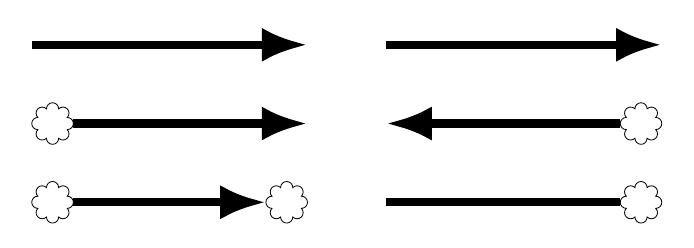
\begin{tikzpicture}[baseline={(current bounding box.center)}]
  \draw[-Latex, line width=3pt]
	(0,1) -- (3.5,1);
  \draw[{Cloud[fill=white]}-Latex, line width=3pt]
    (0,0) -- (3.5,0);
  \draw[{Cloud[fill=white]}-{Latex[].Cloud[fill=white]}, line width=3pt]
    (0,-1) -- (3.5,-1);
   \draw[-Latex, line width=3pt]
   (4.5,1) -- (8,1);
  \draw[Latex-{Cloud[fill=white]}, line width=3pt]
    (4.5,0) -- (8,0);
  \draw[-{Cloud[fill=white]}, line width=3pt]
    (4.5,-1) -- (8,-1);
\end{tikzpicture}

\end{document}
